\documentclass[12pt]{scrartcl}
\usepackage[ngerman]{babel}


\usepackage{amsmath, amssymb}

\usepackage{array}  % for the tables

\usepackage{nameref}  % for referencing with name

\usepackage{hyperref}  % for hyperlinks

\usepackage{mathrsfs}

\usepackage{graphicx}  % for the images

\usepackage{xcolor, colortbl}

\usepackage{gensymb} % for \degree

\usepackage{pgfplots}

\usepackage{tabto}

\usepackage{lipsum} % for the lipsum text

\usepackage{listings}

\usepackage{textcomp} % permille

% Define custom colors
\definecolor{codegreen}{rgb}{0,0.6,0}
\definecolor{codegray}{rgb}{0.5,0.5,0.5}
\definecolor{codepurple}{rgb}{0.58,0,0.82}
\definecolor{backcolour}{rgb}{0.95,0.95,0.92}

% Define custom style for Python code
\lstdefinestyle{pythonstyle}{
    backgroundcolor=\color{backcolour},
    commentstyle=\color{codegreen},
    keywordstyle=\color{magenta},
    numberstyle=\tiny\color{codegray},
    stringstyle=\color{codepurple},
    basicstyle=\ttfamily\footnotesize,
    breakatwhitespace=false,
    breaklines=true,
    captionpos=b,
    keepspaces=true,
    numbers=left,
    numbersep=5pt,
    showspaces=false,
    showstringspaces=false,
    showtabs=false,
    tabsize=2
}

\lstset{style=pythonstyle}


\RedeclareSectionCommand[beforeskip=1cm]{section}
\RedeclareSectionCommand[beforeskip=0.5cm]{subsection}

\newcolumntype{P}[1]{>{\centering\arraybackslash}p{#1}}

\usetikzlibrary{arrows}

% \usepgfplotslibrary{external}

% \tikzexternalize

\definecolor{Gray}{gray}{0.85}

\setlength{\parindent}{0cm}

% hyperlinks
\hypersetup{
    colorlinks,
    citecolor=black,
    filecolor=black,
    linkcolor=black,
    urlcolor=black
}

\bibliographystyle{IEEetran}




\author{David Jäggli}

\title{Zusammenfassung Krypto}



% ---------- Begin Main Document ----------- %



\begin{document}

\maketitle

\tableofcontents

\newpage
\section{Allg}

Allgemeine Begriffe und Definitionen.


\subsection{Terminologie}


\renewcommand{\arraystretch}{1.5}
\begin{center}
    \begin{tabular}{ | m{12em} | m{25em} | }
        \hline
        \textbf{Kryptographie}          & Entwerfen von Krypto-Algorithmen                          \\
        \hline
        \textbf{Kryptoanalyse}          & Brechen von Krypto-Algorithmen                            \\
        \hline
        \textbf{Perfekte Sicherheit}    & Unendlich viele Ressourcen sind equivalent zu raten       \\
        \hline
        \textbf{Unkeyed Kryptographie}  & Hashfunktionen                                            \\
        \hline
        \textbf{Symmetrische Krypt.}    & Beide den gleichen Schlüssel - $\mathcal{O}(n^2)$         \\
        \hline
        \textbf{Asymmetrische Krypt.}   & Öffentlicher und privater Schlüssel - $\mathcal{O}(n)$    \\
        \hline
        \textbf{Stromchiffren}          & Verschlüsselung von einzelnen Zeichen                     \\
        \hline
        \textbf{Blockchiffren}          & Verschlüsselung von Blöcken                               \\
        \hline
        \textbf{MAC}                    & Message Authentication Code                               \\
        \hline
        \textbf{DES}                    & Data Encryption Standard                                  \\
        \hline
        \textbf{EC}                     & Elliptic Curve                                            \\
        \hline
        \textbf{ECC}                    & Elliptic Curve Cryptography                               \\
        \hline
        \textbf{CA}                     & Certificate Authority                                     \\
        \hline
        \textbf{CRL}                    & Certificate Revocation List - Zertifikatssperrliste                                     \\
        \hline
        \textbf{Mutual}                 & Two-way Authentication. Beide Parteien authentifizieren sich                                     \\
        \hline
        \textbf{EWF (mit) Trapdoor}     & Es existert Geheimnis (Trapdoor) mit der sich $f^{-1}(y)$ 
                                            einfach berechnen lässt. Die Sicherheit ist, dass dieser "Trick" \space
                                            nur einer Partei bekannt ist.                                     \\
        \hline
    \end{tabular}
\end{center}


\newpage
\subsection{Trapdoor Weiterführung}

Untenstehend sind die Unterschiede von Einwegfunktionen mit und ohne Trapdoor näher 
erläutert.

\subsubsection{Einwegfunktion ohne Trapdoor}

Beispiele und Erläuterungen für Einwegfunktionen ohne Trapdoor:

\begin{itemize}
    \item Diffie-Hellman $y = f(x) = a^x \mod p$.
    \begin{itemize}
        \item $p$ prim ist rechenintensiv aber einfach.
        \item Das Inverse (disk. Log.) $x \equiv f^{-1}(x) \equiv \log_a(y) \mod p$ 
        ist für alle schwierig.
    \end{itemize}
    \item Elliptische Kurven
    \begin{itemize}
        \item Multiplikation $Q = k \cdot P$, $k$ eine unbekannte Zahl, $P$,$Q$ bekannte
        Punkte.
        \item Das Bestimmen von $k$ aus $Q = k \cdot P$ ist für alle schwierig.
        \item Die Punkt-Division von $\displaystyle{k = \frac{Q}{P}}$ gibt es in diesem Sinne nicht.
    \end{itemize}
\end{itemize}



\subsubsection{Einwegfunktion mit Trapdoor}

Beispiele und Erläuterungen für Einwegfunktionen mit Trapdoor:

\begin{itemize}
    \item Bei RSA: Die e-te Wurzel mod N berechnen: Trapdoor
    \begin{itemize}
        \item Das Potenzieren $y = f(x) \equiv x^e \mod N$ ist rechenintensiv aber einfach.
        \item Das Inverse $x \equiv f^{-1}(x) \equiv y^{1/e} \equiv \sqrt[e]{y} \mod N$ ist extrem schwierig.
        \item Das Berechnen der ``e-ten Wurzel mod N''  ist das eine Problem, das
                Faktorisieren von $N = p \cdot q$ das andere. Der RSA kann gebrochen werden, wenn
                nur eines der zwei Probleme gelöst ist. 
    \end{itemize}
\end{itemize}



\newpage
\section{Schutzmechanismen}

Kleine Übersicht:
\begin{figure}[ht]
    \centering
    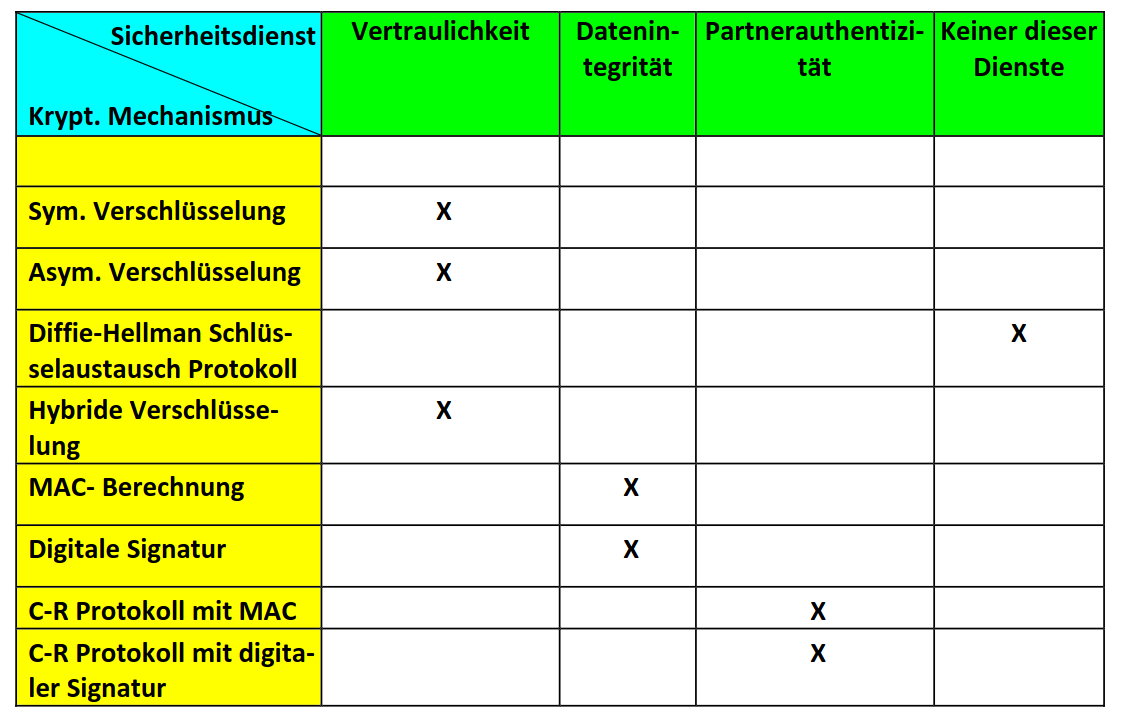
\includegraphics[width=\textwidth]{img/mechanismus_vs_sicherheitsdienst.png}
    \caption{Mechansimus vs Sicherheitsdienst}
    \label{fig:mechanismus_vs_sicherheitsdienst}
\end{figure}

\subsection{Sicherheitsanforderungen}

\begin{itemize}
    \item Vertrauchlichkeit (Abhören)
    \item Integrity (Daten Verändern)
    \item Insertion (Daten Einfügen)
    \item Non repudiation of origin (Abstreiten die Meldung geschickt zu haben)
    \item Replay (Abfangen und wieder senden)
    \item Delete 
    \item Non repudiation of receipt (Abstreiten die Meldung erhalten zu haben)
    \item Authentisierung
\end{itemize}

\subsection{Geheimhaltung / Verschlüsselung}


$K_e$ = Key Encrypt \\
$K_d$ = Key Decrypt \\


Ist $K_e = K_d$ $\rightarrow$ symmetrische Verschlüsselung.\\
Ist $K_e \neq K_d$ $\rightarrow$ asymmetrische Verschlüsselung.


\subsection{Authentizität}

$K_g$ = Key Generate \\
$K_v$ = Key Verify \\

Ist $K_g = K_v$ $\rightarrow$ MAC.\\
Ist $K_g \neq K_v$ $\rightarrow$ digitale Signatur.


\newpage
\label{sec:symmetrische_kryptographie}
\section{Symmetrische Kryptographie}

Note: Stromschiffren bieten keine Integrität.\\
Note: Blockchiffren bieten Integrität.\\
Ausserdem können Blockchiffren verwendet werden für:
\begin{itemize}
    \item Hashfunktionen
    \item Pseudo random number generators
    \item Message Authentication Code (MAC)
\end{itemize}


\subsection[Blockschiffren]{Beschreibung von Blockchiffren}

Grundsätzlicher Ablauf/Aufbau:

\begin{enumerate}
    \item n-Bit Inputblockgrösse
    \item n-Bit Outputblockgrösse
    \item k-Schlüsselbit
    \item x-Verschlüsselungsdurchläufe
\end{enumerate}

übliche Blockgrössen: 64, 128, 256 Bit \\
Anzahl Runden: 10, 12, 14, 16 \\
Übliche Schlüssellängen: 
k = 56 (DES), 112 (3DWS\_2key), \\
k = 128 (AES), 168 (3DES\_3key) \\
k = 192, 256 (AES) Bit\\


\subsubsection[Blockschiffren Eig.]{Eigenschaften von Blockchiffren}

\begin{enumerate}
    \item (Gleicher Schlüssel) Änderung eines Input bits ändert die Hälfte der Outputbits
    \item (Gleicher Input) Änderung eines Schlüsselbits ändert die Hälfte der Outputbits
    \item Mit Binomialkoeffizent kann gezeigt werden, dass diese Eigenschaften ideal sind.
\end{enumerate}

Allgemein ist folgender Binom Ideal wenn $m = n/2$:

$$ \binom{n}{m} = \frac{n!}{m! \cdot (n-m)} $$


\subsubsection{Good to know}

\begin{itemize}
    \item 3DWES\_2key (112 Bit Schlüssellänge) hat Sicherheit von 57-60 Bit
    \item 3DES\_3key (168 Bit Schlüssellänge) hat Sicherheit von 112 Bit
    \item AES braucht für 128 Bit 10 Runden, für 192 Bit 12 Runden und für 256 Bit 14 Runden
    \item AES braucht für Entschlüsselung doppelt so lange wie für Verschlüsselung
    \item AES hat nicht den gleichen Algorithmus für Ver-/Entschlüsselung
    \item PRESENT ist optimiert für 8-Bit Prozessor (IoT)
    \item PRESENT braucht weniger Energie, SW \& HW
\end{itemize}


\subsection{Stromchiffren}

XOR - Ziemlich straight forward, aufgrund von Key wird ein Pseudo-Random Sequence generiert, mit
der dann der Plaintext verschlüsselt (XORd) wird. Entschlüsselung genau gleich

Abkürzungen:
C = Cipher \\
M = Message \\
S = Sequence \\

\textbf{Verschlüsselung:} $C = M \oplus S$ \\
\textbf{Entschlüsselung:} $M = C \oplus S = (M \oplus S) \oplus S = M \oplus (S \oplus S) = M \oplus 0 = M$ \\


\textbf{Charakteristiken:}
\begin{itemize}
    \item Keygenerator
    \begin{itemize}
        \item (Bankenwelt) of ein Blockverschlüssler
        \item (Netwerkwelt) of spezielle Konstruktion mit Hashfunktionen wie SHA-1
    \end{itemize}
    \item Symmetrisch
    \item Vor allem bei Link-Verschlüssler als HW erhlältlich.
    \item Keine Authentizität/Integrität
    \item Ein Verändern im Chiffretext verändert nur die betroffenen Zeichen
    \item Wird jedoch ein Bit hinzugefügt oder entfernt, ist die Hölle los
\end{itemize}

\subsubsection{One-Time-Pad (OTP)}

True-random Key, welcher gleich lang ist wie der Plaintext $\rightarrow$ perfekte Sicherheit.\\

OTP ist eine Stromchiffre, nicht jede Stromchiffre ist ein OTP.



\subsubsection{XOR}

Zwei gleiche Ausdrücke XORen ergibt 0.

\textbf{Beispiel:}  \\
$6B \oplus A5 = CE$ = $(6 XOR A)(B XOR 5)$


\subsubsection{Beurteilung von Stromchiffren}

\begin{enumerate}
    \item Schutzziele: Schutz gegen das Abhören der Meldung
    \item Mit was für Typen / Angriffen muss gerechnet werden: gegen intelligente Gegner, welche 
    passiven Angriff (abhören) durchführen
    \item Stromchiffre Mechanismus: Symmetrische Verschlüsselung
\end{enumerate}


\subsection{Blockchiffren}

Guess what, verschlüsseln immer einen Block und hängen diese hintereinander.


\subsubsection{ECB-Modus für mehrere Blöcke}

Electronic Code Book Mode, einfach alle Blöcke einzeln verschlüsseln.

$$C_i = E(M_i,K)$$

Gleiche Blöcke ergeben gleiche Chiffretexte.


\subsubsection{CBC-Modus für mehrere Blöcke}

Cipher Block Chaining, XOR des vorherigen Chiffretextes (oder IV) mit dem Plaintext.
Respektive braucht einen IV (Initialisierungsvektor) für den ersten Block. Danach dient
der Chiffretext des vorherigen Blocks als IV für den nächsten Block.

$$C_i = E(M_i \oplus C_{i-1}, K) \text{ mit } C_0 = IV$$


Gleiche Blöcke ergeben nicht mehr gleiche Chiffretexte.\\

Wenn die Länge des Plaintextes nicht durch die Blockgrösse teilbar ist, muss der letzte Block
anders behandelt werden. Zum Beispiel einfach abschneiden. Die Entschlüsselung ändert nicht.\\
Die Formel für den letzen Block ist: $C_4 = E(C_3,K) \oplus M_4$


\subsubsection{OFB-Modus = Output Feedback Mode}

Ist grundsätzlich eine Stromchiffre. Hier wird Blockchiffre wird nur als Zufallszahlengenerator verwendet.

\begin{figure}[ht]
    \centering
    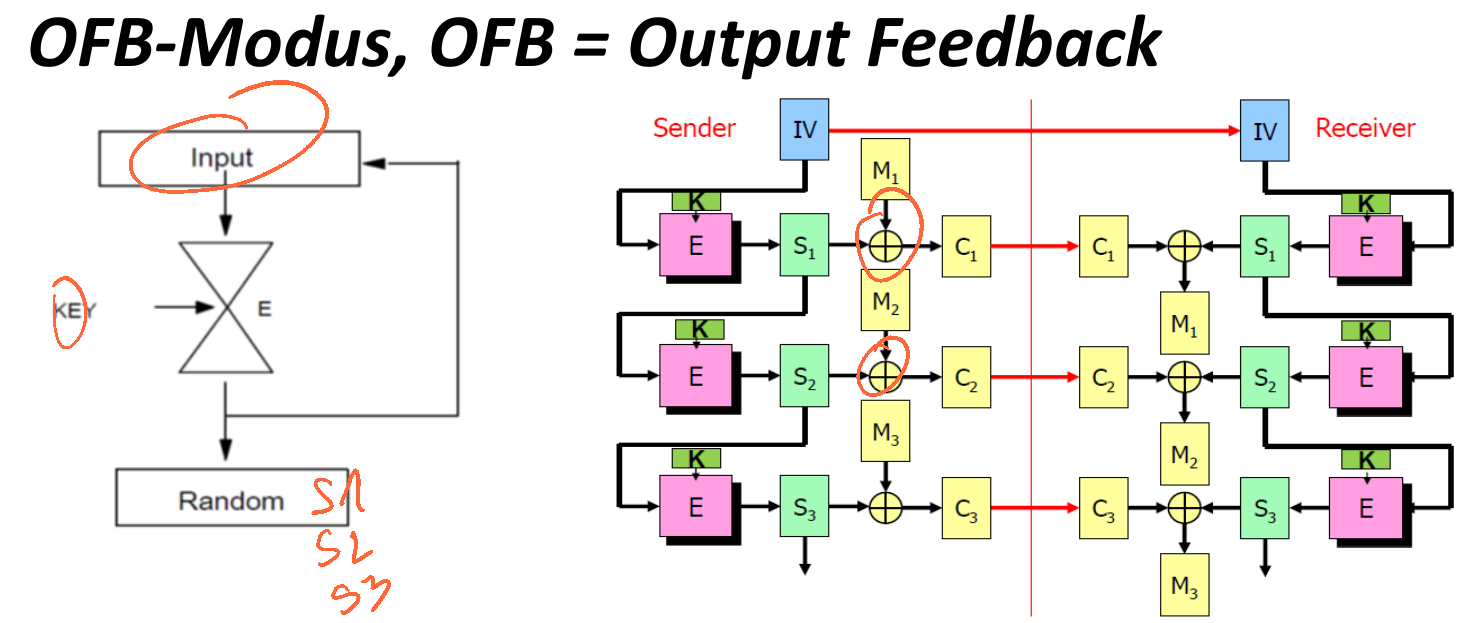
\includegraphics[width=\textwidth]{img/ofb_mode.png}
    \caption{OFB Mode}
    \label{fig:ofb_mode}
\end{figure}

Verschlüsseln:
$$C_i = S_i \oplus M_i \text{ mit } S_i = E(S_{i-1},K) \text{ und } S_0 = IV$$

Entschlüsseln:
$$M_i = S_i \oplus C_i \text{ mit } S_i = E(S_{i-1},K) \text{ und } S_0 = IV$$




\subsubsection{CTR-Modus (Counter Mode)}

Der XOR Schlüssel ist nicht mehr der vorherige (verschlüsselte) Block sondern einfach $IV + i$.

Hat Vorteile von beiden:
\begin{enumerate}
    \item Ist parallelisierbar
    \item Verschlüsselung eines grossen Files / Harddisk möglich
    \item Gleicher Klartext ergibt nicht gleicher Output
    \item Vorausberechnung von Schlüsselmaterial ist möglich
    \item Vertauschen von Chiffratblöcken ist nicht mehr einfach.
\end{enumerate}


\begin{figure}[ht]
    \centering
    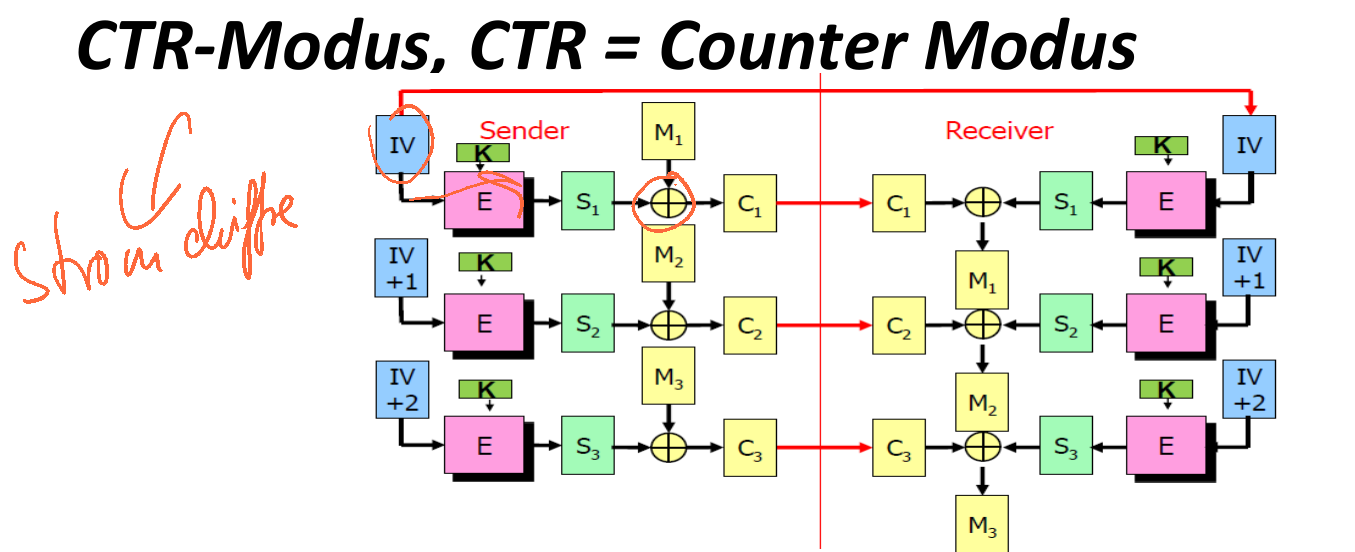
\includegraphics[width=\textwidth]{img/ctr_mode.png}
    \caption{CTR Mode}
    \label{fig:ctr_mode}
\end{figure}


Mathematische Form: $C_i = S_i \oplus M_i$ mit $S_i = E(IV + (i - 1),K)$


\subsection{Auswirkungen bei Bit Manipulation im Chiffretext}


\begin{figure}[ht]
    \centering
    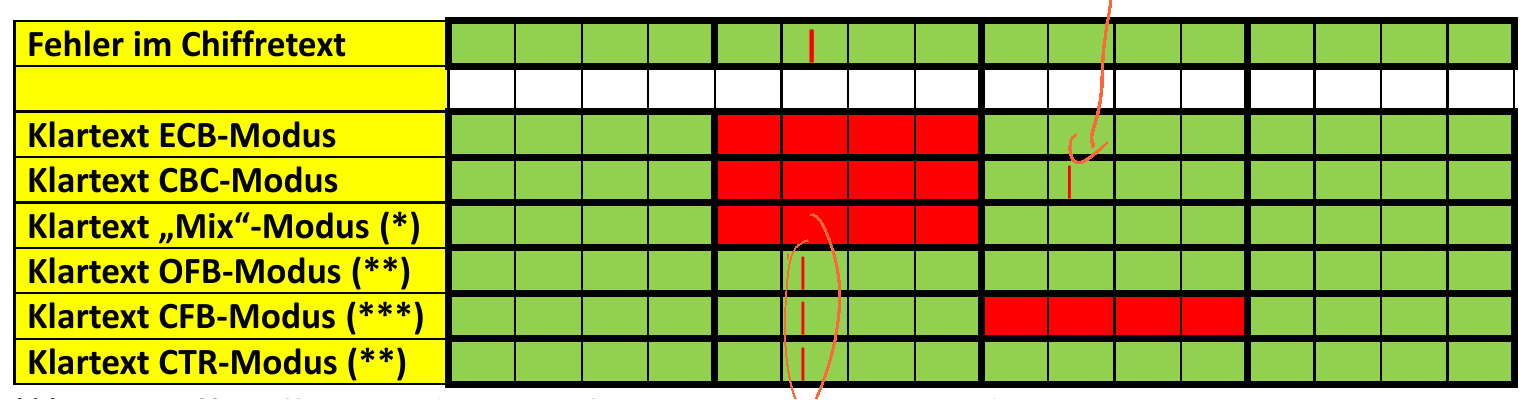
\includegraphics[width=\textwidth]{img/klartext_fehler_nach_manipulation.png}
    \caption{Auswirkung auf Klartext bei Bit Manipulation im Chiffretext}
    \label{fig:auswirkungen_manipulation}
\end{figure}


\subsection{Integritätsschutzmechanismen}

% TODO: (maybe) some more clarity about MACs & HMACs

MAC \& HMAC sind Integritätsschutzmechanismen.\\

MAC halt irgendwie mit CBC oder CTR Mode und HMAC mit Hashing Algorithmus.\\




\newpage
\section{Asymmetrische Kryptographie}

\subsection{Allgemein}

Sicherheitsvergleich klassisch:
\renewcommand{\arraystretch}{1.5}
\begin{center}
    \begin{tabular}{ | m{11em} | P{4em} | P{4em} | P{4em} | P{4em} | P{4em} | P{4em} |}
        \hline
        \textbf{Symmetric}   & \textbf{56}    & \textbf{80}    & \textbf{112}   & \textbf{128}   & \textbf{192}   & \textbf{256}   \\
        \hline
        \textbf{RSA $n$  }   & 512   & 1024  & 2048  & 3072  & 7680  & 15360     \\
        \hline
        \textbf{ECC $p$  }   & 112   & 160   & 224   & 256   & 384   & 512     \\
        \hline
        \textbf{Key-Ratio}   & 5:1   & 6:1   & 9:1   & 12:1  & 20:1  & 30:1     \\
        \hline
    \end{tabular}
\end{center}


\vspace{0.5cm}
Sicherheit mit Quantencomputer:
\begin{enumerate}
    \item Für Faktorosierung bei RSA $K$ braucht ca $2k$ Qubits
    \item Für DL bei ECC von $k$-Bits brauchts ca. $K \approx 5k + 8 \sqrt{k} + 4 \cdot \log_2(k)$ Qubits
\end{enumerate}



\newpage
\subsection{Einwegpermutationen}

RSA, ECC und Diffie-Hellman sind genau genommen Einwegpermutationen.\\

Die Farben blau, grün und rot kann man auf 3! = 6 Arten anordnen:

\begin{center}
    (B, G, R), (B, R, G), (G, B, R), (G, R, B), (R, B, G), (R, G, B)    
\end{center}


Im RSA-System: \\
$N = 3 \cdot 11$ und $e = 13 \Rightarrow d = 13^{-1} \mod \varphi(N) = 17 = 13^{-1} \mod 20$ \\

Nun kann man alle Werte $x \in \mathbb{Z}_{33} = \{0, \dots, 32\}$ mit $y \equiv x^{13} \mod 33$ berechnen
verschlüsseln.\\

\vspace{0.5cm}
\textbf{Beispielaufgabe:}\\
Die 3-stellige Zahl $x$ wird mit der Formel $y \equiv (a \cdot x + b ) \mod N$ verschlüsselt. Die 
Entschlüsselungsfunktion lautet: $x \equiv a^{-1} \cdot (y - b) \mod N$. Dabei ist $N = 11 \cdot 23 \cdot 41$ 
ein Produkt von drei Primzahlen; der Wert $N$ ist öffentlich bekannt. Die Werte $a$ und $b$ bilden in der Form $(a; b)$ 
den geheimen Schlüssel. Die Werte $a$ und $b$ sind für die Verschlüsselung und Entschlüsselung geeignete Werte aus
der Menge $\{2; 3; \dots ; N - 1\}$\\

Aus wie vielen möglichen Schlüsseln der Form $(a; b)$ können bei dieser Verschlüsselung ausgewählt werden? 
Es ist die exakte Zahl anzugeben.\\

Allgemein:\\
\begin{itemize}
    \item Für $b$ sind alle möglichen Werte aus der Menge $\{2;3;\dots;N-1\}$ erlaubt. Das sind $N-2$ Möglichkeiten.
    \item Für $a$ sind aus der Menge $\{2;3;\dots;N-1\}$ alle Werte erlaubt, die teilerfremd zu $N$ sind. Da die Zahl 1
            aber nicht drin sein darf lautet die Anzahl der möglichen Werte für a somit:
            $\varphi(N) - 1 = \varphi(r \cdot s \cdot t) - 1 = \varphi(r) \cdot \varphi(s) \cdot \varphi(t) - 1 = (r-1) \cdot (s-1) \cdot (t-1) - 1$
    \item somit gibt es total $(N-2) \cdot [(r-1) \cdot (s-1) \cdot (t-1) - 1]$ Möglichkeiten
\end{itemize}


\vspace{0.5cm}
Mit Zahlen:\\
$r = 11; s = 23; t = 41 \Rightarrow N = 11 \cdot 23 \cdot 41 = 10'373$\\

$\Rightarrow N -2 = 10'371$\\
$\Rightarrow \varphi(N) - 1 = \varphi(r \cdot s \cdot t) -1 = (11 - 1) \cdot (23 - 1) \cdot (41 - 1) - 1 = 10 \cdot 22 \cdot 40 - 1 = 8'799$\\


\newpage
\subsection{Elliptic Curve Cryptography (ECC)}

\begin{itemize}
    \item Was: mathematische Objekte, die man als Public-Key Kr. verwenden kann
    \item Warum:
    \begin{itemize}
        \item wenige und schnelle Operationen (statt viele langsame wie RSA) wegen 
        multiplikationen statt exponentiationen 
        \item wenig Speicherplatz (für Chipkarten ein Kriterium)
        \item Es gibt Standards
        \item Patent-freie Algorithmen
    \end{itemize}
    \item Man kann:
    \begin{itemize}
        \item Signieren
        \item Schlüsselaustauschen
        \item Hybrid Verschlüsseln
        \item (Wie RSA)
    \end{itemize}
    \item Könnte RSA aufgrund der langen Schlüssel ablösen (vielleicht auch Quantenalgorithmen)
    \item Es wird addiert und verdoppelt statt multipliziert und potenziert (RSA)
    \item Anzahl der Punkte kann Atome im Weltall übertreffen
    \item Ist eine Einwegfunktion ohne Trapdoor
    \item Die Sicherheit liegt im diskreten Logarithmus Problem
    \item Diskreter Logarithmus: für $P,Q$ bei $q = i \cdot P$ kann $i$ nicht einfach berechnet werden
    \item Der Schnittpunkt des Koordinatensystems ist $P(0,0)$, $P(0,0)$ kann Inhalt von EC sein.
    \item Der unendlich Ferne Punk $\mathcal{O}$ ist das neutrale (null-)Element
    \item Die Gruppenordnung ist Anzahl der Punkte (somehow NICHT $p$)
    \item Für gleiche Sicherheit: Ein 3072 Bit RSA entspricht etwa einer 256 Bit EC.
\end{itemize}


\newpage
\subsubsection{Requirements}

Hat immer die Form:

\[ y^2 = x^3 + ax + b \]

und ist NICHT

\[ y = f(x) \]


Nichtsingularitätsbedingung:

\[ 4a^3 + 27b^2 \not\equiv 0 \mod p \]

Diese muss erfüllt sein, ansonsten gibt es mehrere Wurzeln (Ergebnisse).\\
Und ist sie erfüllt, hat die Kurve sowas wie eine Spitze oder Überschneidungen.\\


Diese beiden Bedingungen stellen sicher, dass die Verbindung zwischen zwei Punkten genau
einen weiteren Punkt schneidet. Bei Tangenten wird der Berührpunkt doppelt gezählt.

% \newpage
% \textbf{Beispiel:}

% \begin{figure}[ht]
%     \centering
%     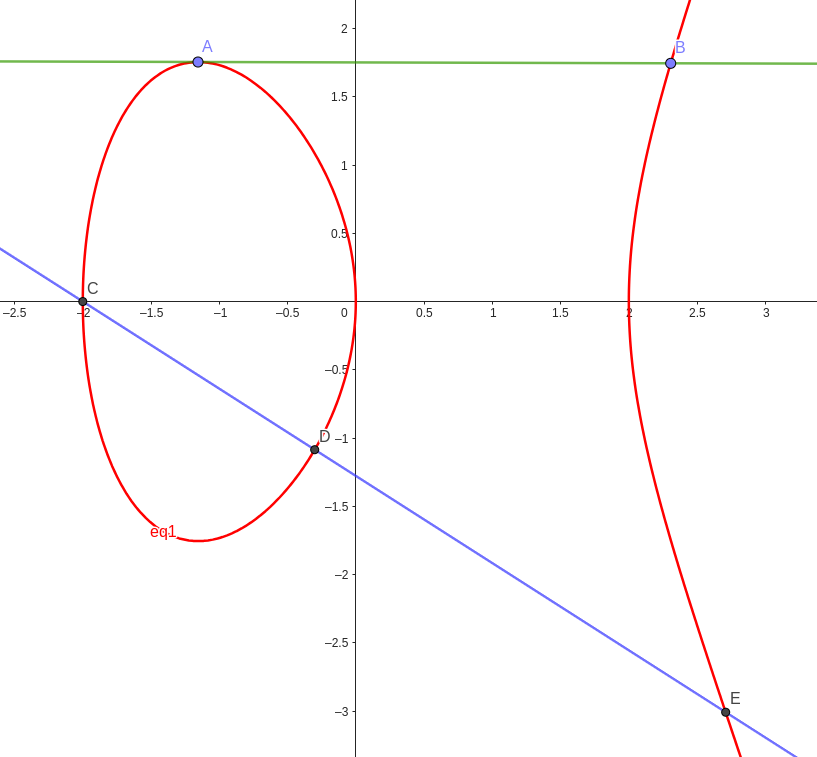
\includegraphics[width=\textwidth]{img/elliptic_curve.png}
%     \caption{Elliptic Curve Beispiel}
%     \label{fig:elliptic_curve}
% \end{figure}

% \[ y^2 = x^3 - 4x \]


\newpage
\subsubsection{Punktaddition}

\begin{figure}[ht]
    \centering
    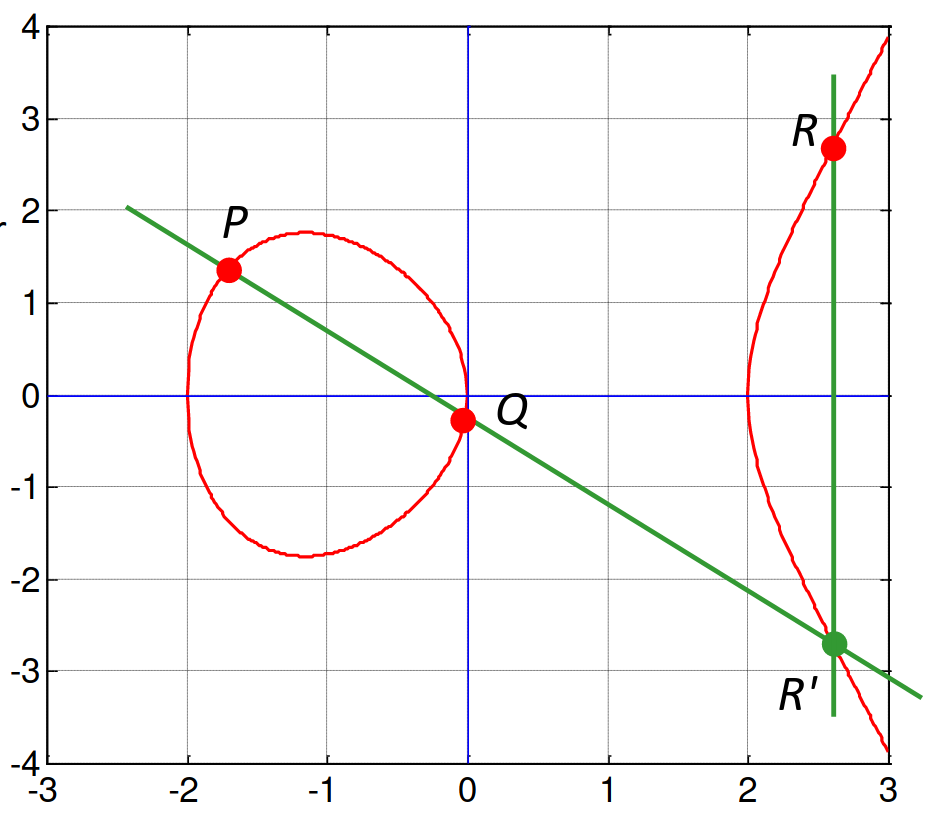
\includegraphics[width=\textwidth]{img/elliptic_curve_addition.png}
    \caption{Elliptic Curve Punkt Addition}
    \label{fig:elliptic_curve_addition}
\end{figure}

\[ P + Q = R \]


\subsubsection{Neutrales und Inverses Element}

Inverses Element resp. Spiegelung an der x-Achse:

\[ P'(x,-y) = -P(x,y) \]

Punktaddition:

\[ P' + P = P + P' = \mathcal{O} \]

Das neutrale Element ist der Punkt im unendlichen, also

\[ \mathcal{O}(x,\infty) \] 

Dann einfach noch die einzelnen Koordinaten mit $p$ modulo rechnen.


\begin{figure}[ht]
    \centering
    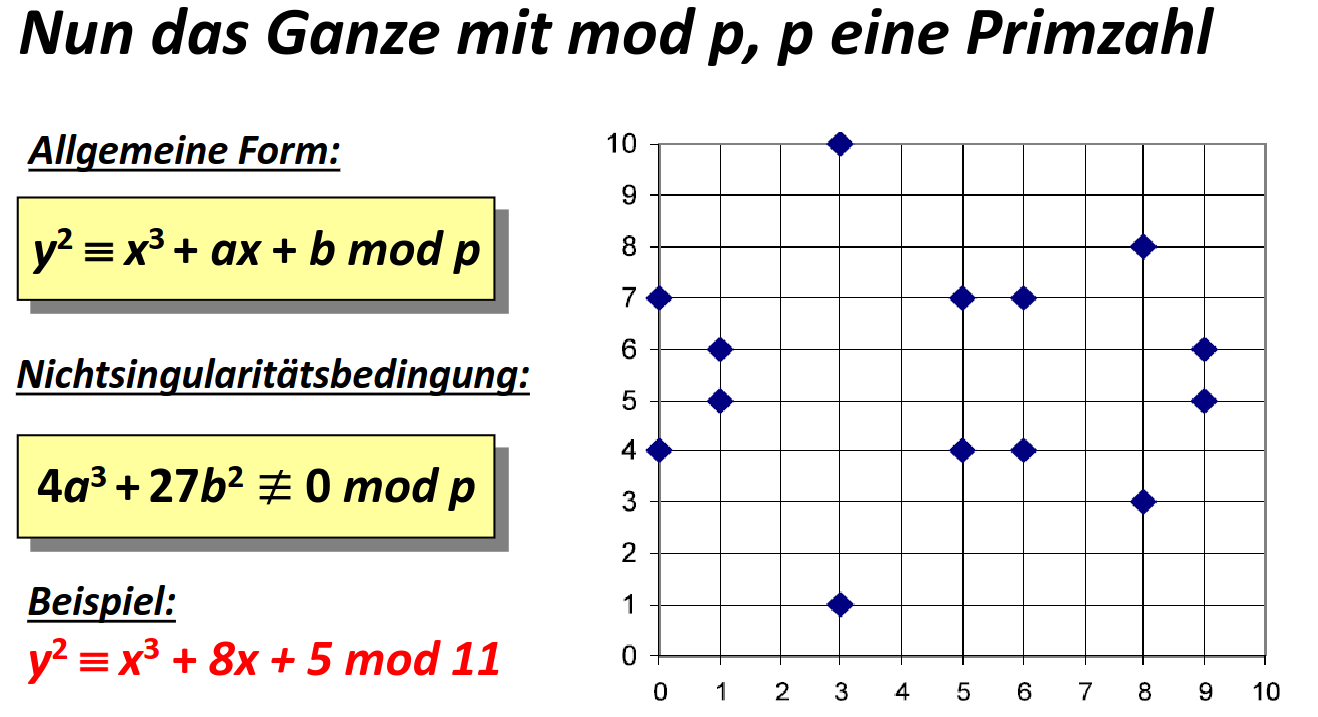
\includegraphics[width=\textwidth]{img/elliptic_curve_mod.png}
    \caption{Elliptic Curve with Modulo}
    \label{fig:elliptic_curve_mod}
\end{figure}

Ein Punkt $P$ mit welchem man alle Punkte ausrechnen kann ist ein Basispunkt. Hier als
Beispiel ($k \cdot $)$P(0,4)$. Wenn wir $P$ mit sich selbst addieren oder den Faktor $k$
vorndran 1,2,3 \dots ausrechnen, erhalten wir alle Punkte der Kurve.\\

Die Koordinaten muss man dabei jweils mit $p$ modulo rechnen.\\

Das $k$ vor dem $P$ muss dan module die Gruppenordnung (wie viele verschiedene 
Punkte dass es gibt) gerechnet werden. Da sich die Punkte wiederholen.



\newpage
\subsubsection{Allgemeine Form \& Zusammenfassung:}

Remember:

\begin{itemize}
    \item allgemeine Form: $E = \{(x;y) | y^2 = x^3 + ax + b \mod p\}$
    \item Nichtsingularitätsbedingung: $4a^3 + 27b^2 \neq 0$
    \item $E$ = Zusammenfassung aller Punkte, welche die Bedingung erfüllen
    \item $p$ muss zwischen 256 und 512 Bit sein
    \item a \& b können beliebig sein, müssen aber die beiden Gesetze erfüllen
    \item Eine Gruppe heist zyklisch wenn es einen erzeugenden Punkt $P$ gibt.
    \item Mit einen eurzeugenden Punkt $P$ kann man alle anderen Punkte erzeugen $k \cdot P$
    \item ist die Gruppenordnung prim $rightarrow$ alle Elemente ausser $\mathcal{O}$ sind erzeugend
\end{itemize}

Bereich der Punkte kann berechnet werden mit: 

\[ p+1 - 2 \sqrt{p} \leq |E| \leq p + 1 + 2 \sqrt{p} \]

Die effektive Range wird durch $a$ und $b$ bestimmt, mit $p$ kann nur die Randzahlen
berechnet werden.


\subsubsection{Formel zur Addition von 2 Punkten}

Zuerst Steigung berechnen, danach können $x$ und $y$ berechnet werden.


\begin{align*}
    s &\equiv \frac{y_2 - y_1}{x_2 - x_1} \mod p \\
    x_3 &\equiv s^2 - x_1 - x_2 \mod p \\
    y_3 &\equiv s(x_1 - x_3) - y_1 \mod p
\end{align*}


\newpage
Falls man P + P (Verdoppelung) rechnen muss, resp wenn $x_1 = x_2;y_1 = y_2$ dann ändert sich die Steigungsformel zu:

\[ s \equiv \frac{3 \cdot x_1^2 + a}{2 \cdot y_1} \mod p \]


Remember: bei $x \cdot y \mod p \equiv (x \mod p \cdot y \mod p) \mod p$

Beispiel mit $P(0;4)$ und $Q(3;1)$ in Kurve $y^2 \equiv x^3 +8x + 5 \mod 11$:

\begin{align*}
    s   &\equiv \frac{1 - 4}{3 - 0}                     \mod 11 \\
        &\equiv \frac{-3}{3}                            \mod 11 \\
        &\equiv (-3) \cdot 3^{-1}                       \mod 11 \\
        &\equiv [(-3) \mod 11 \cdot 3^{-1}  \mod 11]    \mod 11 \\
        &\equiv 8 \cdot 4                               \mod 11 \\
        &\equiv 32                                      \mod 11 = 10
\end{align*}

Danach Punke:

\begin{align*}
    x_3 &\equiv 10^2 - 0 - 3 \mod 11 = 9 \\
    y_3 &\equiv 10 \cdot (0 - 9) - 4 \mod 11 = 5
\end{align*}

\subsubsection{Double and add Algorithmus}

Analog kann zum Square and Multiply Algorithmus effizient gerechnet werden.\\

Beispiel: $28 \cdot P$

\begin{itemize}
    \item $28 = 16 + 8 + 4 = 2^4 + 2^3 + 2^2 = 11100$
    \item Mit der ersten 1 macht man nichts
    \item wegen 1: p $\rightarrow$ 2p $\rightarrow$ 2p + p = 3p $|$ double and add
    \item wegen 1: 3p $\rightarrow$ 6p $\rightarrow$ 6p + p = 7p $|$ double and add
    \item wegen 0: 7p $\rightarrow$ 14p $|$ double
    \item wegen 0: 14p $\rightarrow$ 28p $|$ double
\end{itemize}




\newpage
\subsubsection{Bestimmung aller Punkte}

\begin{figure}[ht]
    \centering
    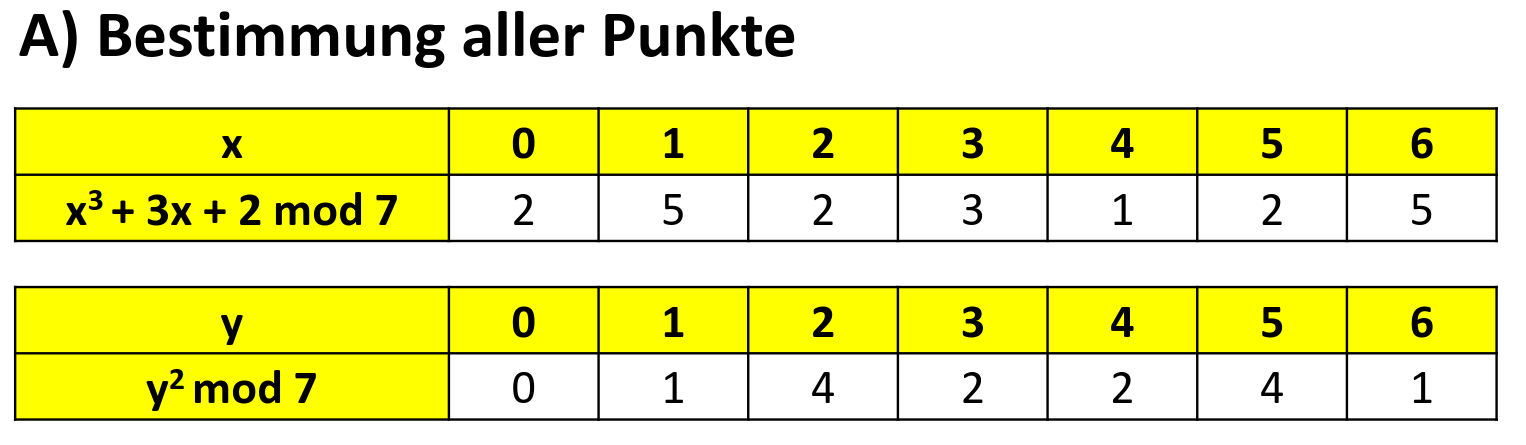
\includegraphics[width=\textwidth]{img/bestimung_aller_punkte.png}
    \caption{Bestimmung aller Punkte}
    \label{fig:bestimmung_aller_punkte}
\end{figure}

Für x = 0: $(0; 3)$ und $(0; 4)$ \\
Für x = 1: keine da $y^2 \mod 7 \neq 5$ \\
Für x = 2: $(2; 3)$ und $(2; 4)$ \\
Für x = 3: keine \\
Für x = 4: $(4; 1)$ und $(4; 6)$ \\
Für x = 5: $(5; 3)$ und $(5; 4)$ \\
Für x = 6: keine \\



\newpage 
\subsubsection{Bestimmung ob Punkt auf Graf ist}

\textbf{Beispiel:}\\

Kurve: $E: \space y^2 \equiv x^3 + x + 1$ über $\mathbb{Z}_{19}$
Punkt : $Q(15, 13)$

\begin{enumerate}
    \item Punkt in Gleichung einsetzen
    \item Links von Gleichung ausrechnen mod p
    \item Rechts von Gleichung ausrechnen mod p
    \item Vergleichen
\end{enumerate}

\begin{align}
    y^2 &\equiv x^3 + x + 1 &&\mod 19 \\
    16^2 &\equiv 15^3 + 15 + 1 &&\mod 19 \\
    16^2 &\equiv 256 &&\mod 19 \equiv 9 \mod 19 \text{ und} \\
    15^3 + 15 + 1 &\equiv 3391 &&\mod 19 \equiv 9 \mod 19
\end{align}

Da beide Seiten gleich sind, ist der Punkt auf der Kurve.



\newpage
\subsection{RSA}

RSA braucht mehr Rechenleistung (ist sicherer?).\\

RSA Keys sind grösser als ECC Keys für gleiche Sicherheit.\\

Ablauf beim Signieren: 

\begin{enumerate}
    \item Hashwert berechnen (Integrität)
    \item Hashwert mit privatem Schlüssel signieren (Authentizität)
\end{enumerate}


\subsubsection{Anzahl der Primzahlen 1-x}

Ist eine Annäherungsformel, berechnet die Anzahl der Primzahlen in $1$ bis $x$ berechnen:

\begin{equation*}
    \pi(x) \approx \frac{x}{\ln(x)} \\
\end{equation*}

Nur ungerade Primzahlen von 1 bis $x$:

\begin{equation*}
    APZ(x) = \frac{Anz. PZ}{Anz. ungerade Z.} \approx \frac{\displaystyle{\frac{x}{ln(x)}}}{ \displaystyle{\frac{x}{2} }} = \frac{2}{ln(x)}\\
\end{equation*}


Beispiel:

\begin{align*}
    \pi(10^{150}) &\approx \frac{10^{150}}{\ln(10^{150})} = \frac{10^{150}}{150 \cdot ln(10)} 
    \approx \frac{10^{150}}{345} \approx \frac{10^{150}}{3.5 \cdot 10^2} = \frac{10 \cdot 10^{149}}{3.5 \cdot 10^2}
    = \frac{10 \cdot 10^{147}}{3.5} \approx 2.9 \cdot 10^{147} \\
    APZ(10^{150}) &\approx \frac{2}{ln(10^{150})} = \frac{2}{150 \cdot ln(10)} \approx \frac{2}{345} = 0.0058 = 0.58\% = 5.8 \text{\textperthousand} \\
\end{align*}



\subsubsection{Anzahl n-stelligen Primzahlen}

Ist die genaue Formel, nicht unbedingt nötig, Annäherungsformel ist genau genug.\\

Anzahl der n-stelligen Primzahlen:

\[ \pi(10^n) - \pi(10^{n-1})  \] \\

Anteil der n-stelligen PZ. in den n-stelligen ungeraden Zahlen:

\begin{equation*}
    APZ(n) = \frac{Anz. PZ}{Anz.ung.Z.} \approx \frac{\pi(10^n) - \pi(10^{n-1})}{\displaystyle{\frac{0.9 \cdot 10^n}{2}}} = \frac{\pi(10^n) - \pi(10^{n-1})}{0.45 \cdot 10^n}
\end{equation*} \\


\textbf{Beispiel:} \\
$n = 150 \Rightarrow x = 10^{150}$ \\

\begin{equation*}
    \pi(10^{150}) - \pi(10^{149}) = \frac{10^{150}}{ln(10^{150})} - \frac{10^{149}}{ln(10^{149})} \approx 2.6 \cdot 10^{147} \\
\end{equation*}


\subsubsection{Dezimalstellen ausrechnen:}

Bits: $N = 1024$\\
$D = N \cdot \log_2(10)$\\
Dezimalstellen: $10^{D} \approx 10^{308}$\\



\newpage 
\subsection{Diskreter Logarithmus bei ECC}

Diffie-Hellman: bei $z \equiv g^x \mod p$ ist auf $x$ schwer zu schliessen.\\
Sofern $p$ minestend 600 stellige Primzahl und $g$ ein Generator ist.\\

Bei EC ist gleichung $Q = k \cdot P$ schwerz auf $k$ zu schliessen.\\





\subsubsection{Key exchange}

Diffie-Hellman (K = Secret): 

\begin{align*}
    A &= g^a \mod p \\
    B &= g^b \mod p \\
    K &= A^b = B^a = g^{ab} \mod p    
\end{align*}

EC Key exchange (K = Secret):

\begin{align*}
    A &= a_{Alice} \cdot P = a_A \cdot P\\
    B &= b_{Bob} \cdot P = b_B \cdot P \\
    K &= b_B \cdot A = (b_B \cdot a_A) \cdot P = a_A \cdot B = (a_A \cdot b_B) \cdot P
\end{align*}


\newpage
\subsection{Verschlüsselung mit EC nach Volker Müller}

\begin{enumerate}
    \item Schlüsselgenerierung (Bob ist Empfänger)
    \begin{enumerate}
        \item Elliptische Kurve wählen
        \item Mit Primzahl ca. 256, 384 oder 512 Bit gross
        \item Koeffizienten a und b wählen
        \item Einem Punkt $P$ der eine zyklische Untergruppe der Primordnung $q$ erzeugt.
        \item $d$ wählen wobei $ 0 < d < q $ und 512 Bit lang
        \item Berechne $Q = d \cdot P$
        \item Damit sind die Beiden Schlüssel erzeugt:
        \begin{itemize}
            \item[] $K_{pub} = (p, a, b, q, P, Q)$ 
            \item[] $K_{priv} = d$
        \end{itemize}
    \end{enumerate}
    \item Verschlüsselung (Sender Alice)
    \begin{enumerate}
        \item Wähle $i$ mit $1 < i < q - 1$
        \item Berechne Einmal-Key $K_E = i \cdot P$
        \item Berechne Masking-Key $K_M = i \cdot Q$
        \item Verschlüssle Meldung $T$ mit $Y = T \oplus x \text{-Wert von } K_M$
        \item Meldung mit Einmal Key schicken also $(Y, K_E)$
    \end{enumerate}
    \item Entschlüsselung (Empfänger Bob)
    \begin{enumerate}
        \item Masking-Key berechnen $K_M = d \cdot K_E$
        \item Meldung entschlüsseln $T = Y \oplus x \text{-Wert von } K_M$
    \end{enumerate}
\end{enumerate}

\newpage
\section{Blinde Signaturen}

Generelle Beschreibung: Anna weis nicht WAS sie unterschreibt, wenn sie das Dokument später sieht,
weis sie aber DASS sie es unterschrieben hat.\\
Nutzen:
\begin{itemize}
    \item Unverfällschbarkeit - kein falsches Geld erzeugen
    \item Anonymität - gegenüber Bank
    \item Unlinkbarkeit - keinen Zusammenhang zwischen $s$ und $m$
\end{itemize}

\vspace{0.5cm}
\noindent
Beispiel-Ablauf:

\begin{enumerate}
    \item Kunde zieht geld ab $m$ ist Identifikationsnummer
    \item Kunde bildet $m'$ und fragt Bank um Unterschrift
    \item Bank rechnet $s'$ aus $m'$ und bucht Geld ab und schickt $s'$ zurück (Signatur)
    \item Kunde berechnet $s$ aus $s'$ für den Wert $m$ 
    \item Kunde bezahlt im Shop mit $m$ und $s$
    \item Shop kann mit Public-Key und Signatur kontrollieren ob von Bank signiert
    \item Shop liefert Geld mit ID $m$ und Signatur $s$ bei Bank ein.
    \item Bank prüft ebenfalls Signatur.
    \item Bank weis nun, dass dieses Geld abgehoben wurde, aber nicht von wem.
\end{enumerate}


\newpage
Allgemeiner mathematischer Ablauf:

\begin{enumerate}
    \item Kunde kenn Public-Key $N$ und $e$
    \item Bank kenn Private-Key $d$
    \item Kunde: Wahl der Nachricht $m \rightarrow$ eindeutige Seriennummer
    \item Kunde: Nachricht "blinden"\text{:}
    \begin{enumerate}
        \item Zufällige wahl von $r \in_R \mathbb{Z}^*_N$
        \item $N = p \cdot q$ mit $p,q$ Primzahlen
        \item $ggT(r,N) = 1$
        \item $ggT(r,N) \neq p$
        \item $ggT(r,N) \neq q$
        \item Berechnung von $m' \equiv r^e \cdot m \mod N$
    \end{enumerate} 
    \item Kunde: "geblindete" Nachricht $m'$ schicken
    \item Bank: Nachricht $m'$ signieren:\\
    $s' \equiv (m')^d \mod N$
    \item Bank: Signatur $s'$ schicken
    \item Kunde: Berechnung der Signatur $s$:\\
    $s \equiv s' \cdot r^{-1} \mod N$
    \item Kunde: Überprüfen der Signatur:\\
    $m \equiv s^e \mod N \rightarrow$ ok?
    \item Kunde: Bezahlen mit $m$ und $s$
    \item Shop und Bank überprüfen Echtheit der Münze nach Schritt 7.
\end{enumerate}


\subsection{Beweis der Korrektheit}

\begin{equation*}
    \frac{s'}{r} \equiv \frac{(m')^d}{r} \equiv \frac{(r^e \cdot m)^d}{r} \equiv \frac{r^{ed} \cdot m^d}{r} \equiv \frac{r \cdot m^d}{r} \equiv m^d \equiv s \mod N
\end{equation*}


\newpage
\subsection{Beispiel mit Zahlen}

\textbf{Parameter:}
\begin{itemize}
    \item Öffentlicher Schlüssel: $(N,e) = (91, 5)$
    \item Privater Schlüssel: $(p,q,d) = (7,13,29)$
\end{itemize}

\textbf{Kontrolle der Paramter:}\\
$\varphi(N) = \varphi(7 \cdot 13) = \varphi(7) \cdot \varphi(13) = 6 \cdot 12 = 72 = (2 \cdot 2 \cdot 2 \cdot 3 \cdot 3)$\\
$e = 5$ ist teilerfremd zu 72.\\
$d = 5^{-1} \mod 72 \equiv 29$, da $5 \cdot 29 \equiv 145 \equiv 2 \cdot 72 + 1 \equiv 1 \mod 72$\\

Sei $m = 11$ die Nachricht.\\
Wir wählen zufällig $r = 16$\\
es muss gelten: $ggT(N,r) = ggT(91,16) = 1$\\

\textbf{Erwartete Signatur:}\\
$s \equiv m^d \mod N \equiv 11^{29} \mod 91 = 72$\\



\begin{figure}[ht]
    \centering
    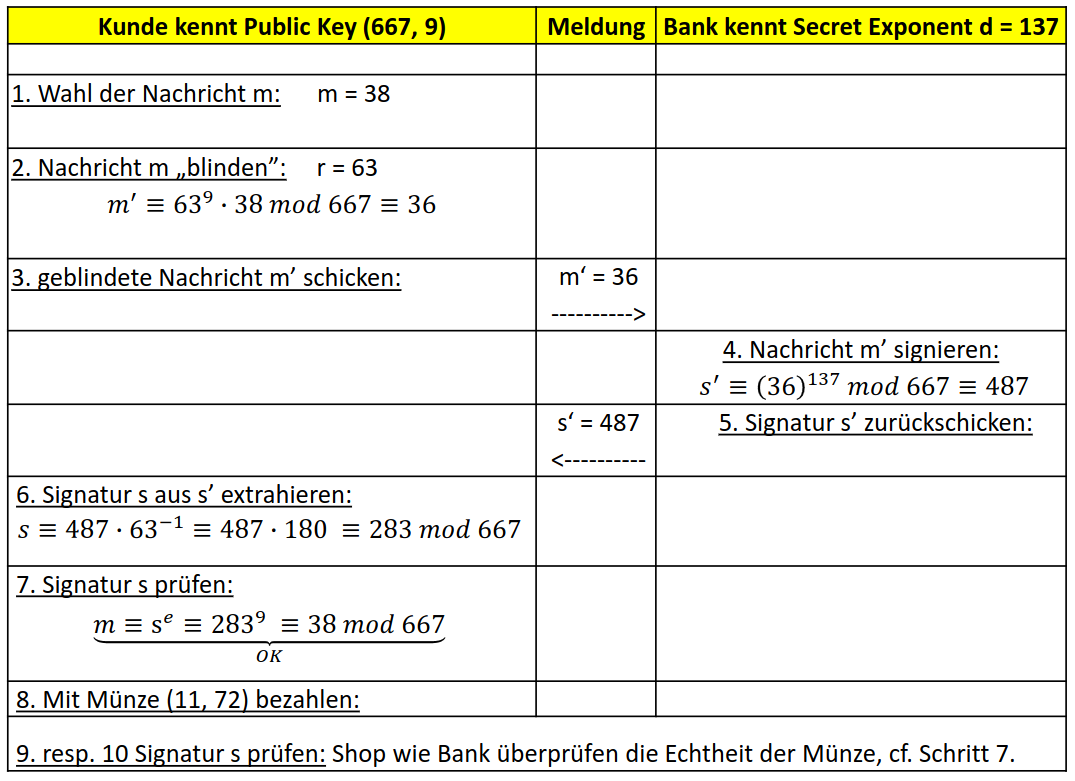
\includegraphics[width=0.9\textwidth]{img/blinde_signatur.png}
    \caption{Blinde Signaturen}
    \label{fig:blinde_signaturen}
\end{figure}


\newpage
\subsection{Basis-Test}

\begin{itemize}
    \item geheimer Exponent muss aufgeteilt werden
    \item Man kann ihn additiv oder multiplikativ aufteilen
    \item Kann beliebig additiv aufgeteilt werden
    \item Kann NICHT beliebig multiplikativ aufgeteilt werden:\\
    Der erste Teil der Aufteilung muss teilerfremd zu $\varphi(N)$ sein, also $ggT(d_1; \varphi(N)) = 1$.
    \item Ablauf der Erstellung einer Doppelsignatur ist bei additiv und multiplikativ nicht dieselbe\\
    Bei multiplikativ muss z.B. die Reihenfolge eingehalten werden.
    \item Blinde Signaturen werden z.B. für anonymes, digitales Geld verwendet.
\end{itemize}




\newpage
\section{Einführung in die Public-Key Infrastruktur (PKI)}

\subsection{Verschlüsseln und Signieren (repetition)}

% TODO: verlinken zu initialem Kapitel

\subsubsection{Verschlüsseln}



\subsubsection{Signieren}

\textbf{Ablauf signieren:}

\begin{enumerate}
    \item Dokument von Alice ist Ausgangswert
    \item Hash berechnen $\rightarrow$ Hashwert
    \item chiffrieren (mit private key und Hash) $\rightarrow$ Signatur
    \item Dokument \& Signatur + Zertifikat $\rightarrow$ signiertes Dokument
\end{enumerate}

Achtung: Schlüsselverwendung bei Signatur ist umgekehrt wie bei Verschlüsselung. Private Key
wird für die Erstellung der Signatur verwendet und Public-Key um zu validieren.\\

Warum Zertifikat? $\rightarrow$ um sicherzustellen, dass der öffentliche Schlüssel auch wirklich
von Alice ist.

\newpage
\textbf{Ablauf Signatur prüfen:}
\begin{enumerate}
    \item Dokument von Alice ist Ausgangswert
    \item Dokument entpacken (Signatur und Dokument)
    \item Signatur mit öffentlichem Schlüssel entschlüsseln $\rightarrow$ Hashwert
    \item Hashwert von Dokument berechnen
    \item Hashes vergleichen
    \item Zertifikat Überprüfen
    \item Wenn alles ok dann ist Signatur gültig.
\end{enumerate}


\subsection{Zertifikate}

\subsubsection{Herstellung eines Zertifikats}


Allgemeiner Ablauf:
\begin{itemize}
    \item Antragssteller identifiziert sich bei CA
    \item Aus dessen Informationen wird Datensatz gebildet (Zertifikatsinhalt)
    \item Datensatz wird mit privatem Schlüssel von CA signiert $\rightarrow$ Zertifikat 
    \item CA veröffentlicht Zertifikat
\end{itemize}


Technisches vorgehen:
\begin{enumerate}
    \item Zertifikatsinhalt
          \begin{itemize}
              \item Version
              \item Serial Number
              \item Subject
              \item Public Key
          \end{itemize}
    \item Inhalt hashen
    \item Hash signieren
    \item Signitierter Hash + Zertifikatsinhalt $\rightarrow$ Zertifikat
\end{enumerate}


\newpage
\subsubsection{Installation eines neues (Root-)Zertifikates}

\begin{enumerate}
    \item Root-CA-Zertifikat Echtheit überprüfen
    \item Echtheitsprüfung wird mit Fingerprint gemacht
    \item Lokal angezeigter Fingerprint wird mit vertrauenswürdiger Referenzquelle verglichen
\end{enumerate}


\subsubsection{Überprüfung der Echtheit eines Zertifikates vom Betriebssystem}

\begin{enumerate}
    \item Applikation überprüft Signatur auf Zertifikat mithilfe des Root-CA-Zertifikates.
    \item Zertifizierungsstelle muss im System hinterlegt sein; sie wird zum Trust Anchor
\end{enumerate}



\subsubsection{Zertifikatsklassen}

\begin{itemize}
    \item \textbf{Klasse 1:} wenig Sicherheit, keine Identitätsprüfung
    \item \textbf{Klasse 2:} mittlere Sicherheit, schwache Identitätsprüfung
    \item \textbf{Klasse 3:} hohe Sicherheit, strenge Identitätsprüfung
    \item \textbf{Qualified Certificate:} höchste Stufe, werden nur für natürliche Personen ausgestellt
\end{itemize}


\newpage
\section{Protokolle}
% TODO: missed some parts until page 22


\subsection{User Authentication}

\begin{itemize}
    \item Username / Password
    \item One-Time Password
    \item Symmetric Algorithms
    \item Public-Key Algorithms
    \item Biometric Authentication
\end{itemize}

\vspace{0.5cm}
\subsection{False-rates}
Es gibt zwei Arten von False-rates:
\begin{itemize}
    \item False Acceptance Rate (FAR)
    \item False Rejection Rate (FRR)
\end{itemize}

Beide sollten so tief wie mögliche sein. Aber es ist ein Tradeoff zwischen den beiden.
Senkt man die Eine erhöht sich die Andere.


\subsection{Verifikationen}
\subsubsection{One to many}
Handy: überprüfe ob ich derjenige bin, der ich vorzugeben behaupte.


\subsubsection{Many to one}
Bank: überprüfe ob ich derjenige bin, der ich vorzugeben behaupte.


\newpage
\subsection{Paralellsession Attacke}
Zwei Sessions eröffnen, dann muss nichts gerechnet werden und Zufalls-/Chiffrierzahl
kann kopiert werden.

\begin{figure}[ht]
    \centering
    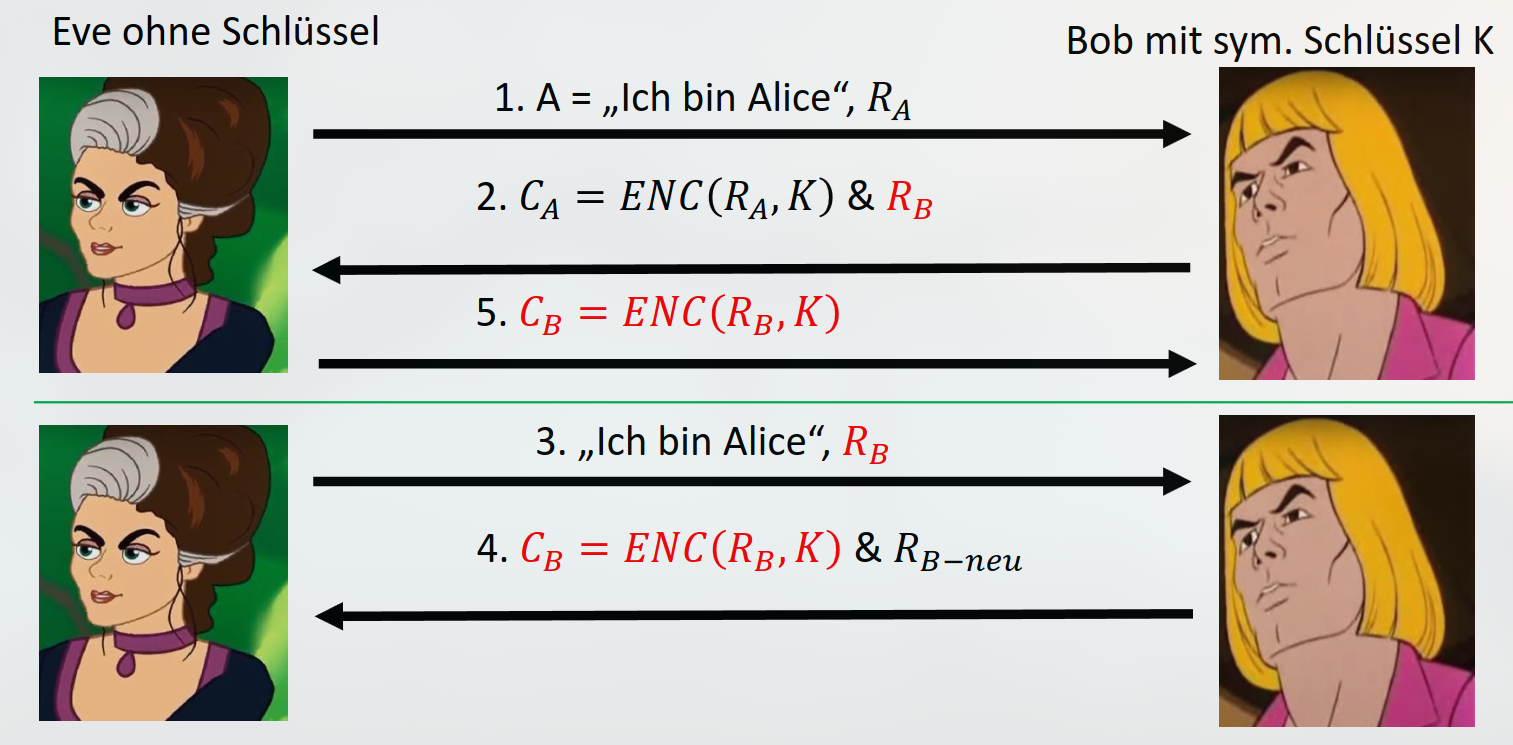
\includegraphics[width=\textwidth]{img/paralell_session_attack.png}
    \caption{Paralellsession Attacke}
    \label{fig:paralell_session_attack}
\end{figure}


\newpage
\section{Quantenkryptographie}

Quantenkryptographie und Quantencomputer sind zwei verschiedene Dinge.

\subsection{Polarization}

4 Zustände, jedem muss 1 oder 0 zugewiesen werden.

\begin{itemize}
    \item Senkrecht
    \item Wagrecht
    \item Schräg links
    \item Schräg rechts
\end{itemize}

Darauf basierend können Filter kreiert werden. Sollte filter nicht auf Teilchen
passen, ist es 50/50 in welchem Zustand es durchgelassen wird.


\subsection{Quantum Key Exchange}

\begin{enumerate}
    \item Sender Alice wählt zufällige Bits
    \item Alice sendet Photonen mit gewählter Polarization
    \item Empfänger Bob wählt zufällige Filter
    \item Bob erhlält gefilterte Photonen
    \item Bob kennt die Kodierung und ordnet 1 oder 0 zu
    \item Bob sendet zurück, welche Filter er benutzt hat
    \item Alice sagt, welche Filter korrekt waren
\end{enumerate}


Im statistischen Mittle werden in 50\% die falschen Filter gewählt. Zudem werden
die Hälfte davon werden aufgedeckt um zu prüfen ob man abgehört wurde. Es müssen
also ca. 4 mal so viele geschickt werden. \\


Key-takeaway: immer die Bits verwenden, welche durch den Filter nicht verändert werden. Alle
anderen haben einen nicht vorhersagbaren Zustand.






% ---------- End Main Document ----------- %


% image example
% \begin{figure}[ht]
%     \centering
%     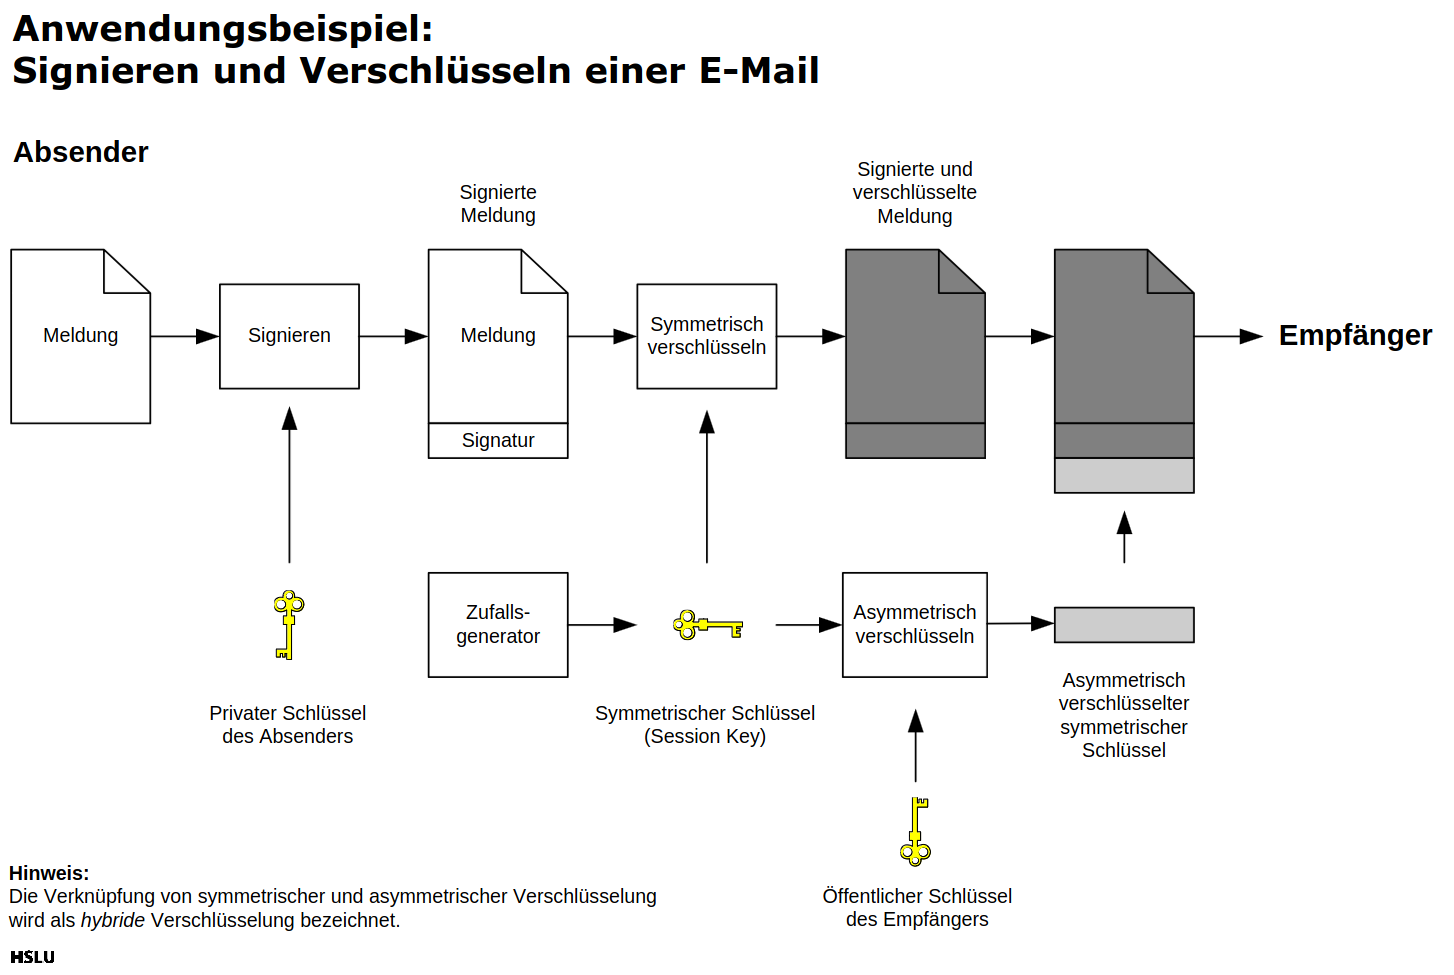
\includegraphics[width=\textwidth]{img/Anwendungsbeispiel_signieren.png}
%     \caption{Anwendungsbeispiel Signieren}
%     \label{fig:your_label}
% \end{figure}



% \begin{align*}
%     587 &= 1 \cdot 392 + 195 \\
% \end{align*}

% Matrix example
% $
% \begin{bmatrix}
%     a_{1,1} & a_{1,2} & a_{1,n}\\
%     a_{2,1} & a_{2,2} & a_{2,n}\\
%     a_{m,1} & a_{m,2} & a_{m,n}
% \end{bmatrix}$\\

% tabular example 3 columns
% \renewcommand{\arraystretch}{1.5}
% \begin{center}
%     \begin{tabular}{ | m{12em} | m{12em} | m{12em} | }
%         \hline
%         1 & 2 & 3\\
%         \hline
%         1 & 2 & 3\\
%         \hline
%         1 & 2 & 3\\
%         \hline
%     \end{tabular}
% \end{center}


% tabular example 2 columns
% \renewcommand{\arraystretch}{1.5}
% \begin{center}
%     \begin{tabular}{ | m{17em} | m{17em} | }
%         \hline
%         1 & 2\\
%         \hline
%         1 & 2\\
%         \hline
%         1 & 2\\
%         \hline
%     \end{tabular}
% \end{center}


% \begin{tikzpicture}[line cap=round,line join=round,>=triangle 45,x=0.5cm,y=0.25cm]
%     \begin{axis}[
%     x=0.75cm,y=0.5cm, % size of the grid
%     axis lines=middle,
%     ymajorgrids=true,
%     xmajorgrids=true,
%     xmin=-10,
%     xmax=10,
%     ymin=-10,
%     ymax=10,
%     xtick={-11,-10,...,10},
%     ytick={-10,-9,...,9},]
%     \draw[line width=2pt,color=blue] () -- (-2,-1);
%     \begin{scriptsize}
%         \draw[color=blue] (-9.866,-4.728) node {$g$};
%         \draw[color=blue] (-1.906,7.172) node {$f$};
%         \draw[color=blue] (3.134,5.232) node {$h$};
%     \end{scriptsize}
% \end{axis}
% \end{tikzpicture}




% \bibliography{quantum_ready}

\end{document}
